\newpage
\section{Thiết kế sơ đồ mạng sử dụng Cisco Packet Tracer}
\subsection{Sơ đồ mạng tổng thể}
\begin{figure}[H]
    \centering
    % Điều chỉnh [width=0.9\textwidth] để ảnh chiếm 90% chiều rộng trang giấy
    % Thay "ten_anh_cua_ban.png" bằng tên file ảnh thực tế của bạn
    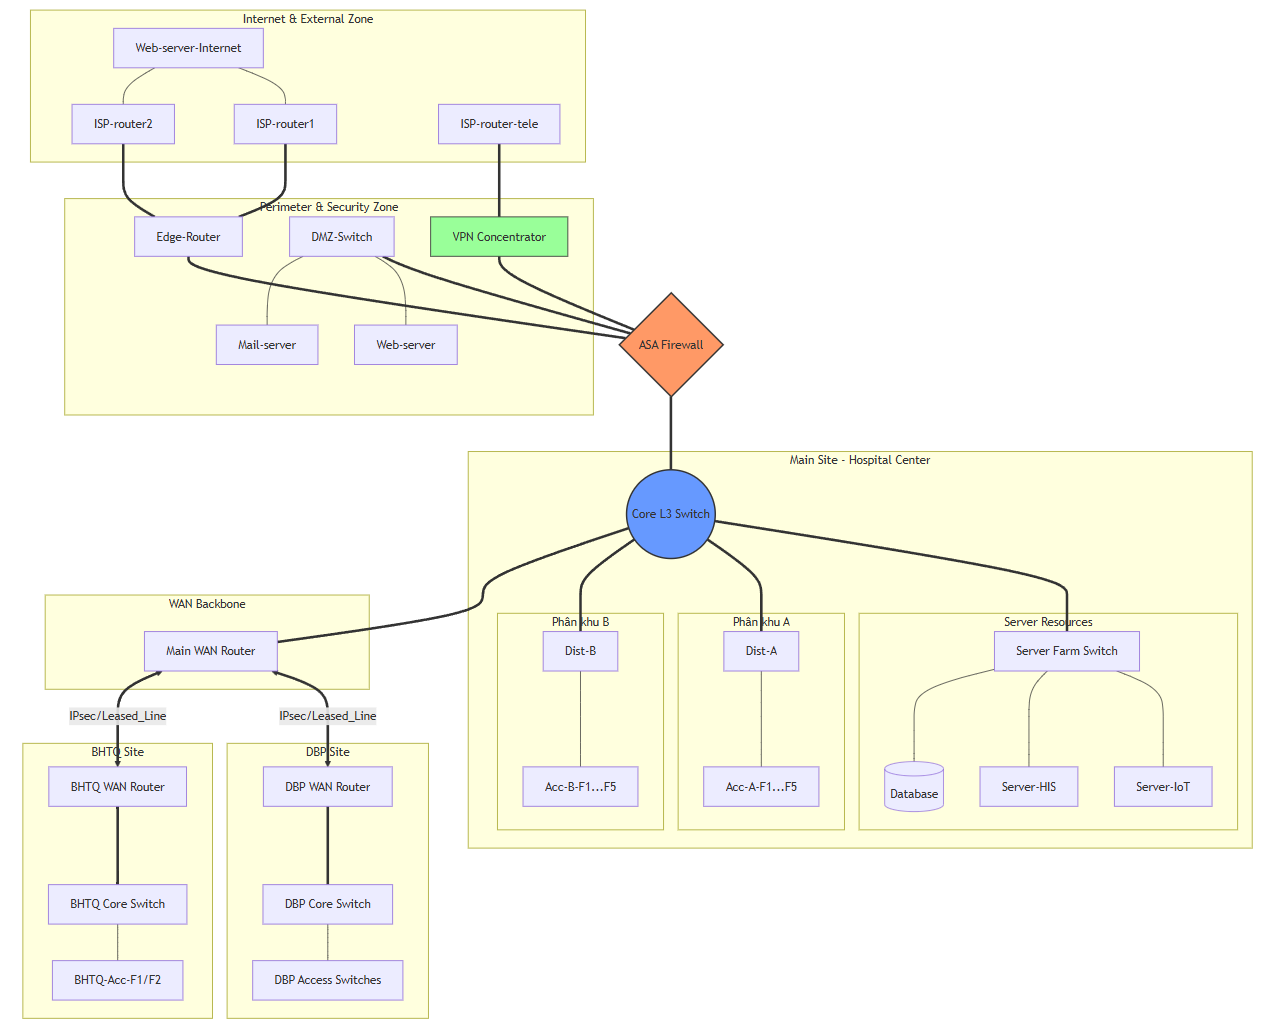
\includegraphics[width=0.9\textwidth]{Pkt_Images/Full-site-UML.png}
    
    % Tiêu đề của ảnh (giống với caption trong báo cáo mẫu)
    \caption{Sơ đồ mạng tổng thể}
    
    % Nhãn để trích dẫn ảnh trong bài (Ví dụ: "Như được thể hiện trong Hình \ref{fig:three_tier}")
    \label{fig:full_site_map}
\end{figure}

\subsection{Sơ đồ mạng tại Data center}
\begin{figure}[H]
    \centering
    % Điều chỉnh [width=0.9\textwidth] để ảnh chiếm 90% chiều rộng trang giấy
    % Thay "ten_anh_cua_ban.png" bằng tên file ảnh thực tế của bạn
    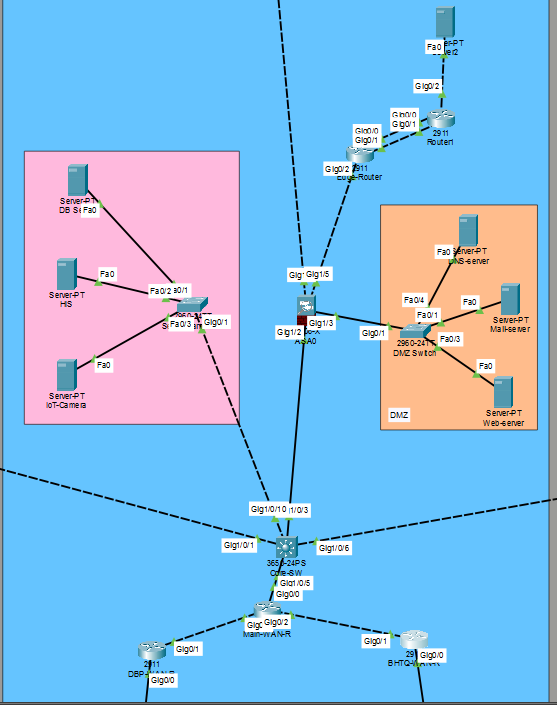
\includegraphics[width=0.4\textwidth]{Pkt_Images/Data-center.png}
    
    % Tiêu đề của ảnh (giống với caption trong báo cáo mẫu)
    \caption{Sơ đồ mạng tại Data center}
    
    % Nhãn để trích dẫn ảnh trong bài (Ví dụ: "Như được thể hiện trong Hình \ref{fig:three_tier}")
    \label{fig:data_center_map}
\end{figure}

\subsection{Sơ đồ mạng tòa A, tòa B tại trụ sở chính}
\begin{figure}[H]
    \centering
    % Hình thứ nhất (bên trái)
    \begin{subfigure}[b]{0.48\textwidth}
        \centering
        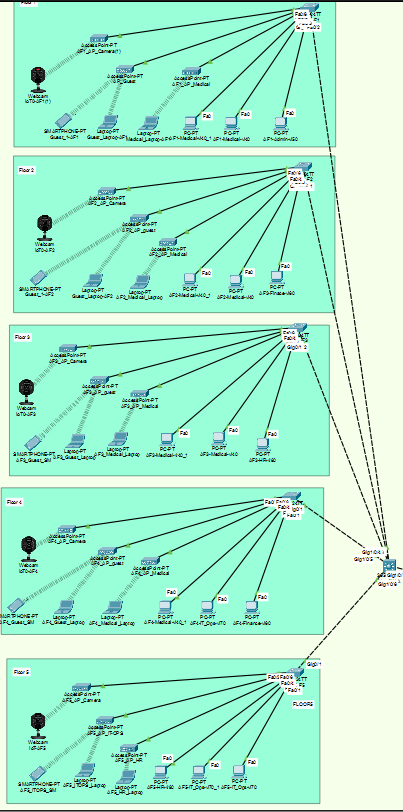
\includegraphics[width=\textwidth]{Pkt_Images/site-A.png}
        \caption{Sơ đồ mạng Tòa A}
        \label{fig:toa_a}
    \end{subfigure}
    \hfill % Tạo khoảng trống tối đa giữa 2 hình
    % Hình thứ hai (bên phải)
    \begin{subfigure}[b]{0.48\textwidth}
        \centering
        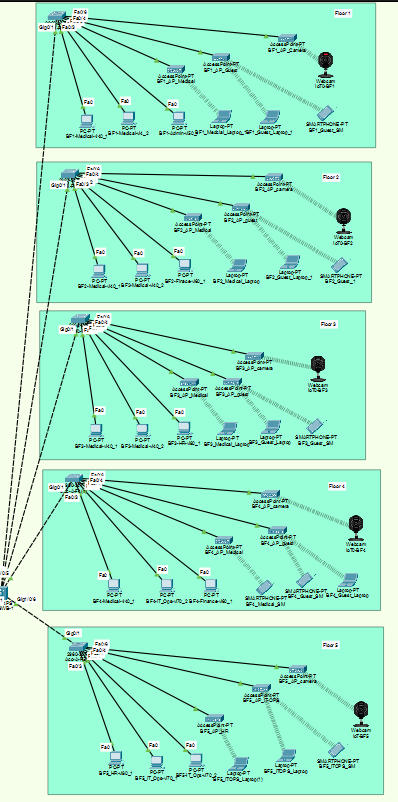
\includegraphics[width=\textwidth]{Pkt_Images/site-B.png}
        \caption{Sơ đồ mạng Tòa B}
        \label{fig:toa_b}
    \end{subfigure}

    \caption{Sơ đồ mạng tòa A và tòa B tại trụ sở chính}
    \label{fig:network_toa_ab}
\end{figure}

\subsection{Sơ đồ mạng tại trụ sở DBP và trụ sở BHTQ}
\subsubsection{Tại trụ sở DBP}
\begin{figure}[H]
    \centering
    % Điều chỉnh [width=0.9\textwidth] để ảnh chiếm 90% chiều rộng trang giấy
    % Thay "ten_anh_cua_ban.png" bằng tên file ảnh thực tế của bạn
    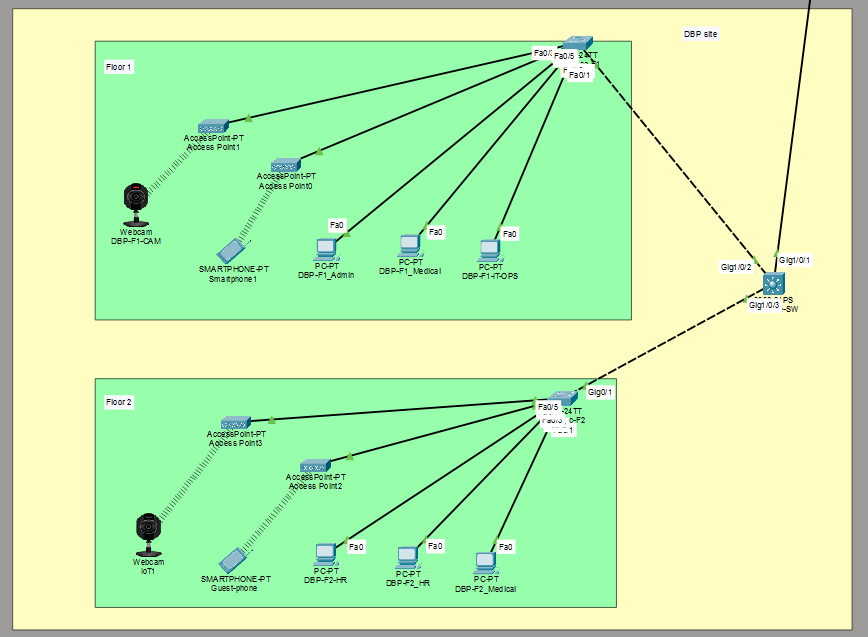
\includegraphics[width=0.6\textwidth]{Pkt_Images/DBP-site.png}
    
    % Tiêu đề của ảnh (giống với caption trong báo cáo mẫu)
    \caption{Sơ đồ mạng tại trụ sở DBP}
    
    % Nhãn để trích dẫn ảnh trong bài (Ví dụ: "Như được thể hiện trong Hình \ref{fig:three_tier}")
    \label{fig:dbp_site_map}
\end{figure}
\subsubsection{Tại trụ sở BHTQ}
\begin{figure}[H]
    \centering
    % Điều chỉnh [width=0.9\textwidth] để ảnh chiếm 90% chiều rộng trang giấy
    % Thay "ten_anh_cua_ban.png" bằng tên file ảnh thực tế của bạn
    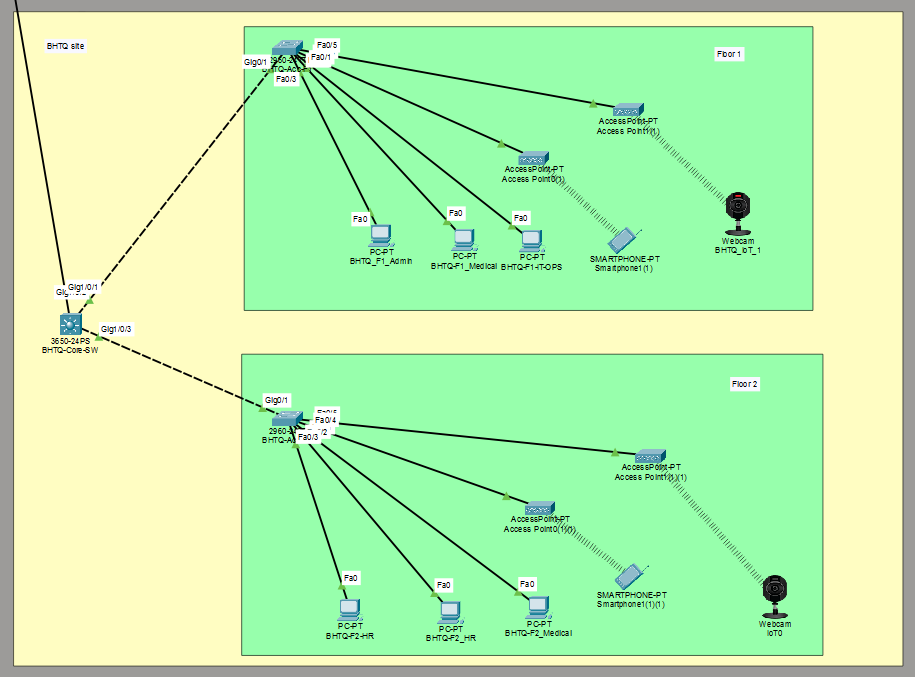
\includegraphics[width=0.6\textwidth]{Pkt_Images/BHTQ-site.png}
    
    % Tiêu đề của ảnh (giống với caption trong báo cáo mẫu)
    \caption{Sơ đồ mạng tại trụ sở BHTQ}
    
    % Nhãn để trích dẫn ảnh trong bài (Ví dụ: "Như được thể hiện trong Hình \ref{fig:three_tier}")
    \label{fig:bhtq_site_map}
\end{figure}

\subsection{Mô tả sơ bộ cho thiết kế hệ thống mạng}

\subsubsection{Phân vùng biên và Bảo mật (Edge \& Security Zone)}
Hệ thống kết nối với Internet thông qua các thiết bị sau:
\begin{itemize}
    \item \textbf{Internet \& External Zone:} Sử dụng đa kết nối ISP (2 đường truyền) để đảm bảo tính dự phòng, một đường truyền riêng (ISP-router-tele) được dành cho kết nối VPN.
    \item \textbf{ASA Firewall:} Đóng vai trò là trung tâm kiểm soát luồng dữ liệu (Hub). Mọi lưu lượng từ bên ngoài vào hệ thống nội bộ hoặc vùng DMZ đều phải đi qua kiểm tra tại đây.
    \item \textbf{Vùng DMZ:} Chứa các Server công cộng như Web-server và Mail-server, được tách biệt với mạng nội bộ qua DMZ-Switch để giảm thiểu rủi ro bị tấn công trực diện vào cơ sở dữ liệu.
    \item \textbf{VPN Concentrator:} Cho phép các kết nối từ xa truy cập an toàn vào hệ thống thông qua các đường truyền được mã hóa.
\end{itemize}

\subsubsection{Cấu trúc mạng tại Trụ sở chính (Main Site)}
Mạng nội bộ tại trụ sở chính được thiết kế theo mô hình 3 lớp tiêu chuẩn:
\begin{itemize}
    \item \textbf{Core Layer (Lớp lõi):} Sử dụng thiết bị \textbf{Core L3 Switch} hiệu năng cao, chịu trách nhiệm chuyển mạch gói tin tốc độ cao giữa các phân khu, Server Farm và kết nối WAN.
    \item \textbf{Distribution Layer (Lớp phân phối):} Gồm các Switch \textbf{Dist-A} và \textbf{Dist-B}, đóng vai trò hội tụ dữ liệu từ các tầng (F1-F5), thực hiện định tuyến và áp đặt các chính sách truy cập (ACLs).
    \item \textbf{Access Layer (Lớp truy cập):} Các Switch truy cập (Acc-A, Acc-B) kết nối trực tiếp với thiết bị đầu cuối của người dùng tại các tầng từ 1 đến 5.
\end{itemize}

\subsubsection{Trung tâm dữ liệu và Máy chủ (Server Farm)}
Các tài nguyên quan trọng được tập trung tại \textbf{Server Farm Switch}:
\begin{itemize}
    \item \textbf{Server HIS:} Hệ thống thông tin bệnh viện (Hospital Information System).
    \item \textbf{Server IoT:} Quản lý dữ liệu từ các thiết bị IoT (Camera).
    \item \textbf{Database (DB):} Hệ quản trị cơ sở dữ liệu dùng chung, được bảo vệ sâu nhất trong cấu trúc mạng.
\end{itemize}

\subsubsection{Kết nối liên chi nhánh (WAN Infrastructure)}
Hệ thống mở rộng kết nối tới các chi nhánh (DBP Site và BHTQ Site) thông qua trục \textbf{WAN Backbone}:
\begin{itemize}
    \item \textbf{Main WAN Router:} Thực hiện kết nối tới các Router chi nhánh thông qua công nghệ \textit{IPsec VPN} hoặc đường thuê riêng \textit{Leased Line}.
    \item \textbf{Tại các chi nhánh:} Sử dụng cấu trúc thu gọn (Collapsed Core) với WAN Router kết nối trực tiếp xuống Core/Dist Switch và tỏa ra các Access Switch, đảm bảo đầy đủ tính năng quản lý.
\end{itemize}


